\documentclass[crop,tikz]{standalone}
\begin{document}
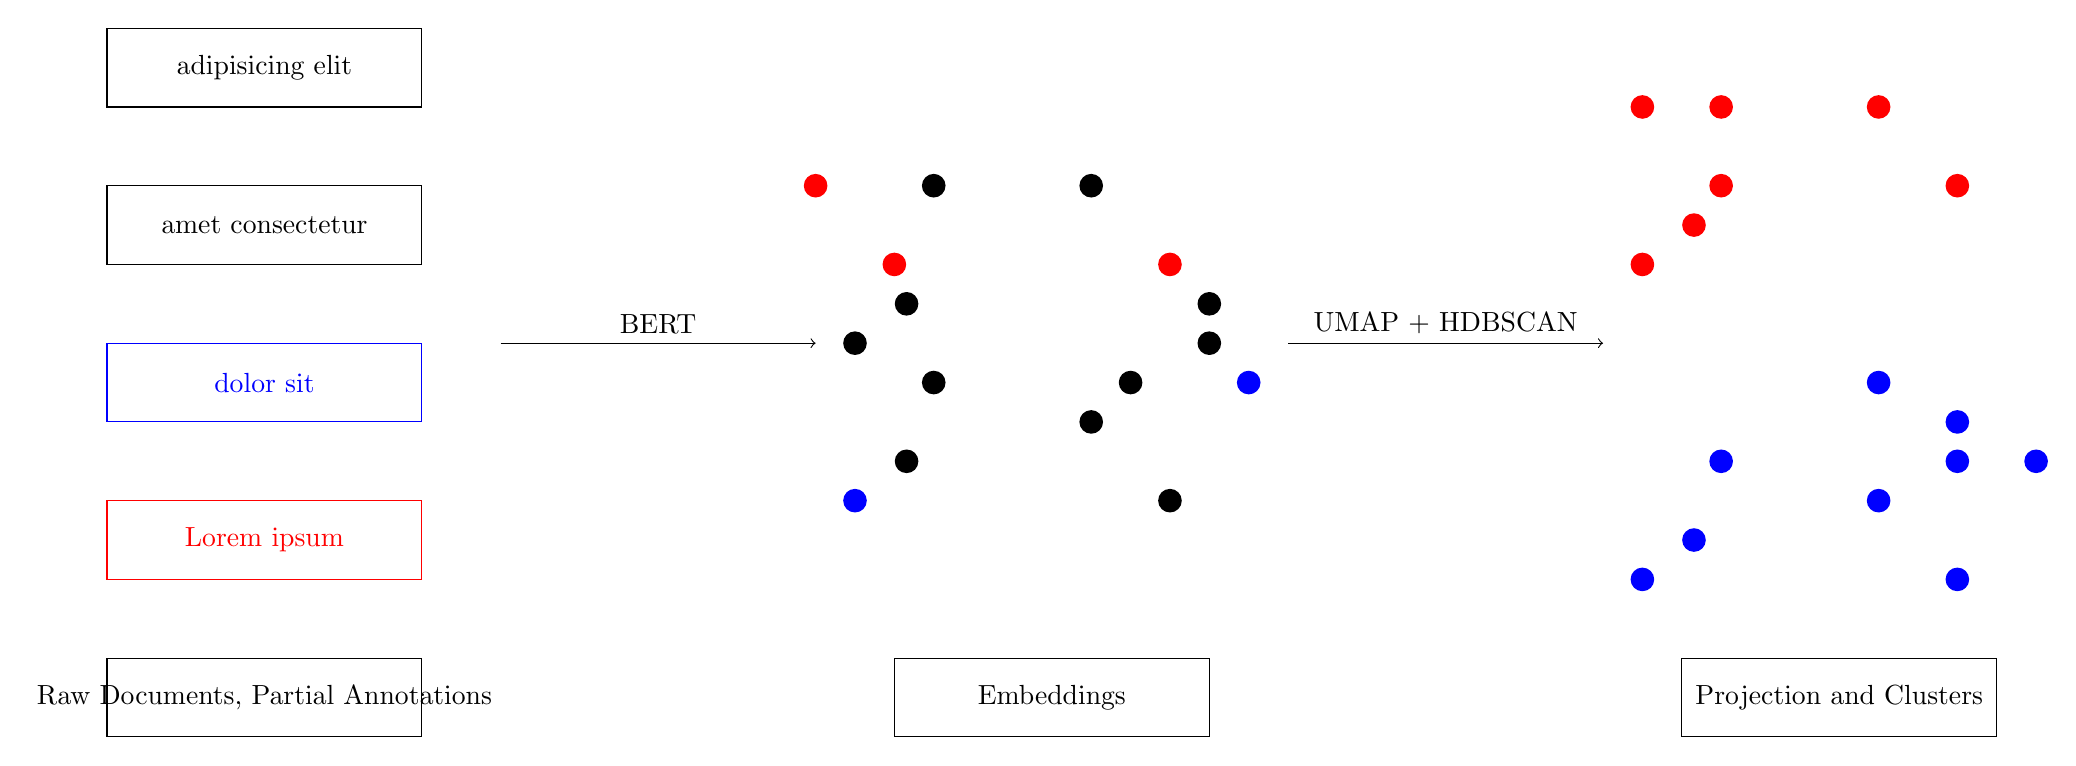
\begin{tikzpicture}

  \draw (0, -2) rectangle (4,-1) node[pos=.5] {Raw Documents\\, Partial Annotations};

  \draw[color=red] (0,0) rectangle (4,1) node[pos=.5] {Lorem ipsum};
  \draw[color=blue] (0,2) rectangle (4,3) node[pos=.5] {dolor sit};
  \draw (0,4) rectangle (4,5) node[pos=.5] {amet consectetur};
  \draw (0,6) rectangle (4,7) node[pos=.5] {adipisicing elit};

  \draw (10, -2) rectangle (14,-1) node[pos=.5] {Embeddings};

  \fill[color=red] (2+8, 4) circle (.15) node {};
  \fill (2+8.5, 5) circle (.15) node {};
  \fill[color=red] (2+7, 5) circle (.15) node {};
  \fill (2+7.5, 3) circle (.15) node {};
  \fill (2+8.155, 3.5) circle (.15) node {};
  \fill (2+8.5, 2.5) circle (.15) node {};
  \fill[color=blue] (2+7.5, 1) circle (.15) node {};
  \fill (2+8.155, 1.5) circle (.15) node {};
  \fill (6+7, 2.5) circle (.15) node {};
  \fill (6+6.5, 5) circle (.15) node {};
  \fill[color=red] (6+7.5, 4) circle (.15) node {};
  \fill (6+8, 3) circle (.15) node {};
  \fill (6+8, 3.5) circle (.15) node {};
  \fill[color=blue] (6+8.5, 2.5) circle (.15) node {};
  \fill (6+6.5, 2) circle (.15) node {};
  \fill (6+7.5, 1) circle (.15) node {};

  \draw (20, -2) rectangle (24,-1) node[pos=.5] {Projection and Clusters};

  \fill[color=red] (12+8.5, 5) circle (.15) node {};
  \fill[color=red] (12+8.5, 6) circle (.15) node {};
  \fill[color=red] (12+7.5, 6) circle (.15) node {};
  \fill[color=red] (12+7.5, 4) circle (.15) node {};
  \fill[color=red] (12+8.155, 4.5) circle (.15) node {};
  \fill[color=blue] (12+8.5, 1.5) circle (.15) node {};
  \fill[color=blue] (12+7.5, 0) circle (.15) node {};
  \fill[color=blue] (12+8.155, .5) circle (.15) node {};

  \fill[color=blue] (16+7.5, 1.5) circle (.15) node {};
  \fill[color=red] (16+6.5, 6) circle (.15) node {};
  \fill[color=red] (16+7.5, 5) circle (.15) node {};
  \fill[color=blue] (16+7.5, 2) circle (.15) node {};
  \fill[color=blue] (16+6.5, 2.5) circle (.15) node {};
  \fill[color=blue] (16+8.5, 1.5) circle (.15) node {};
  \fill[color=blue] (16+6.5, 1) circle (.15) node {};
  \fill[color=blue] (16+7.5, 0) circle (.15) node {};


  \draw[->] (5, 3) -- (9, 3) node[pos=.5, anchor=south] {BERT};
  \draw[->] (15, 3) -- (19, 3) node[pos=.5, anchor=south] {UMAP + HDBSCAN};

\end{tikzpicture}
\end{document}